The restricted Boltzmann machine is up and running and the hyperparamters has been optimized for the different system sizes. We will now thoroughly test the machines accuracy over the different system variables. Each system's ground state energy evolves differently, and that may affect the machine's accuracy, as well as the gap between the ground state and first excited state and the distance from the initialized machine state. For each system we will go through each variable in turn and see how the machine accuracy evolves with it. Following we will do a comparison of the computation time between the restricted Boltzmann machine and diagonalization of the Hamiltonian matrix through Numpy\cite{harris2020array}.

\chapter{The Lipkin model}
\section{The Lipkin model}
\subsection{The effect of \texorpdfstring{$\varepsilon$}{epsilon} on RBM prediction accuracy}
\subsection{The effect of \texorpdfstring{$V$}{V} on RBM prediction accuracy}
\subsection{The effect of \texorpdfstring{$W$}{W} on RBM prediction accuracy}
\subsection{Comparing computation time with diagonalization}


\chapter{The Ising model}
\section{The Ising model}


\begin{figure}[H]
  \begin{center}
    \includegraphics[width=0.95\textwidth]{Figures/Plots/Ising/Result14conv}
  \end{center}
  \caption{The convergence graph of the RBM mean energy output for the Ising model with $N = 14$ particles, $M=1$, and $J=-1$ and $L=-0.5$.}
\end{figure}

The two-dimensional Ising model results in the following convergence graph:

\begin{figure}[H]
  \begin{center}
    \includegraphics[width=0.95\textwidth]{Figures/Plots/Ising/Result9conv}
  \end{center}
  \caption{The convergence graph of the RBM mean energy output for the two-dimensional Ising model with $N = 3$ particles, $M=3$, and $J=-1$ and $L=-0.5$.}
\end{figure}

\subsection{The effect of \texorpdfstring{$J$}{J} on RBM prediction accuracy}

\begin{figure}[H]
  \begin{center}
    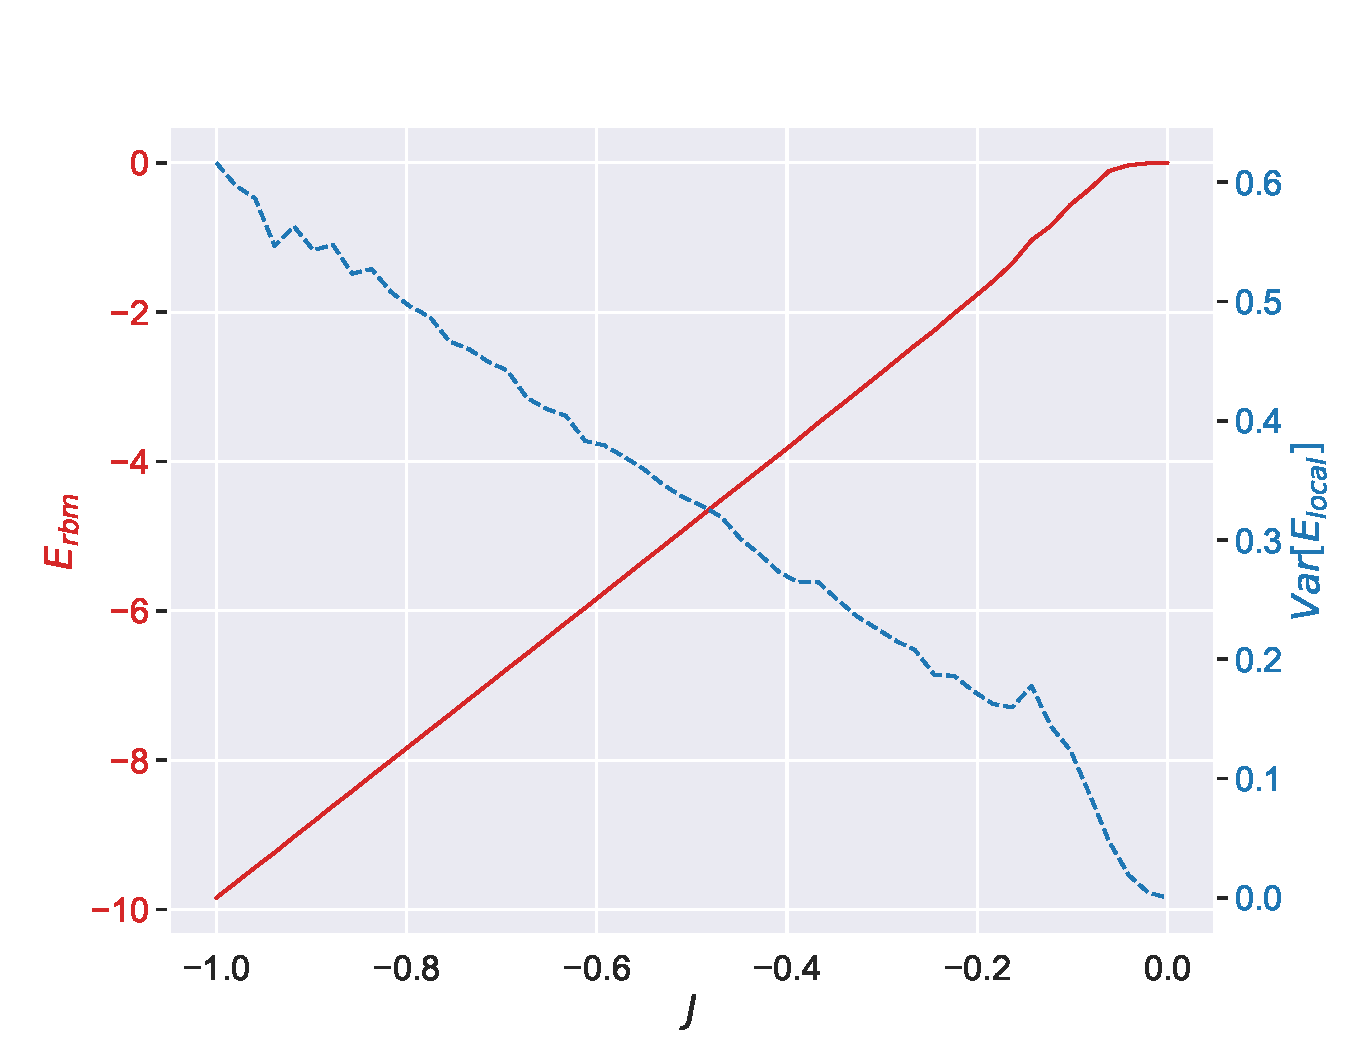
\includegraphics[width=0.95\textwidth]{Figures/Plots/Ising/[J][-1.0-0.0][e=500][n=10][L=0]}
  \end{center}
  \caption{The variance of the restricted Boltzmann machine local energy output for the Ising model with $10$ lattice points and $L=0$.}
\end{figure}


\begin{figure}[H]
  \begin{center}
    \includegraphics[width=0.95\textwidth]{Figures/Plots/Ising/[J][-1.0-0.0][e=500][n=10][L=-0.5]}
  \end{center}
  \caption{The variance of the restricted Boltzmann machine local energy output for the Ising model with $10$ lattice points and $L=-0.5$.}
\end{figure}

Looking at the two-dimensional version we get

\begin{figure}[H]
  \begin{center}
    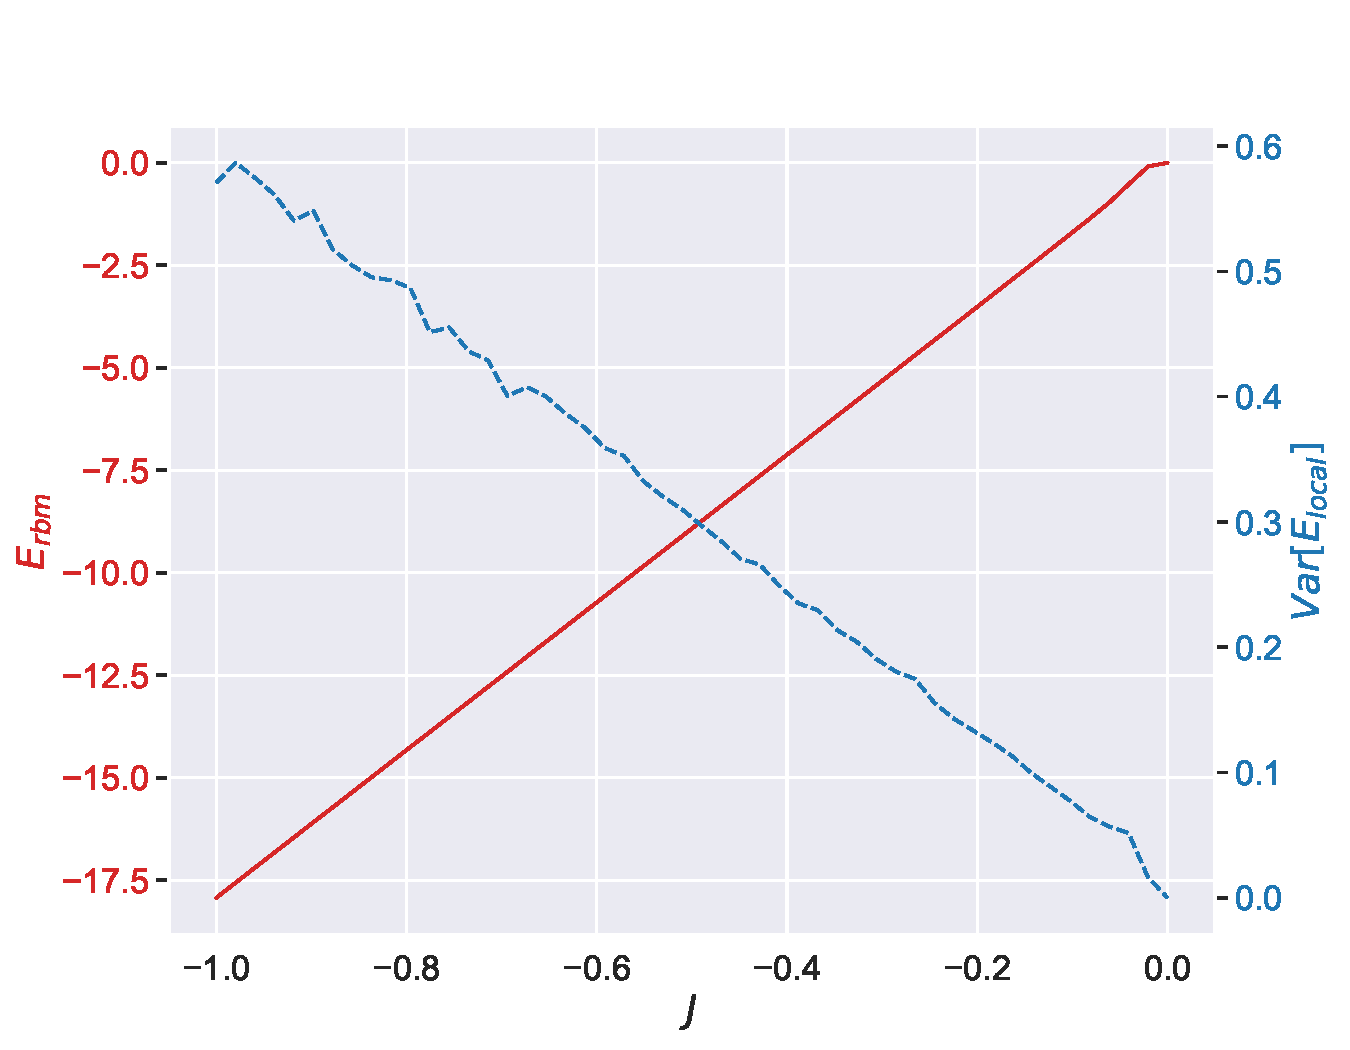
\includegraphics[width=0.95\textwidth]{Figures/Plots/Ising/[J][-1.0-0.0][e=500][n=9][L=0]}
  \end{center}
  \caption{The variance of the restricted Boltzmann machine local energy output for the two=two-dimensional Ising model with $9$ lattice points, $N=3$ and $M=3$, and $L=0$.}
\end{figure}


\begin{figure}[H]
  \begin{center}
    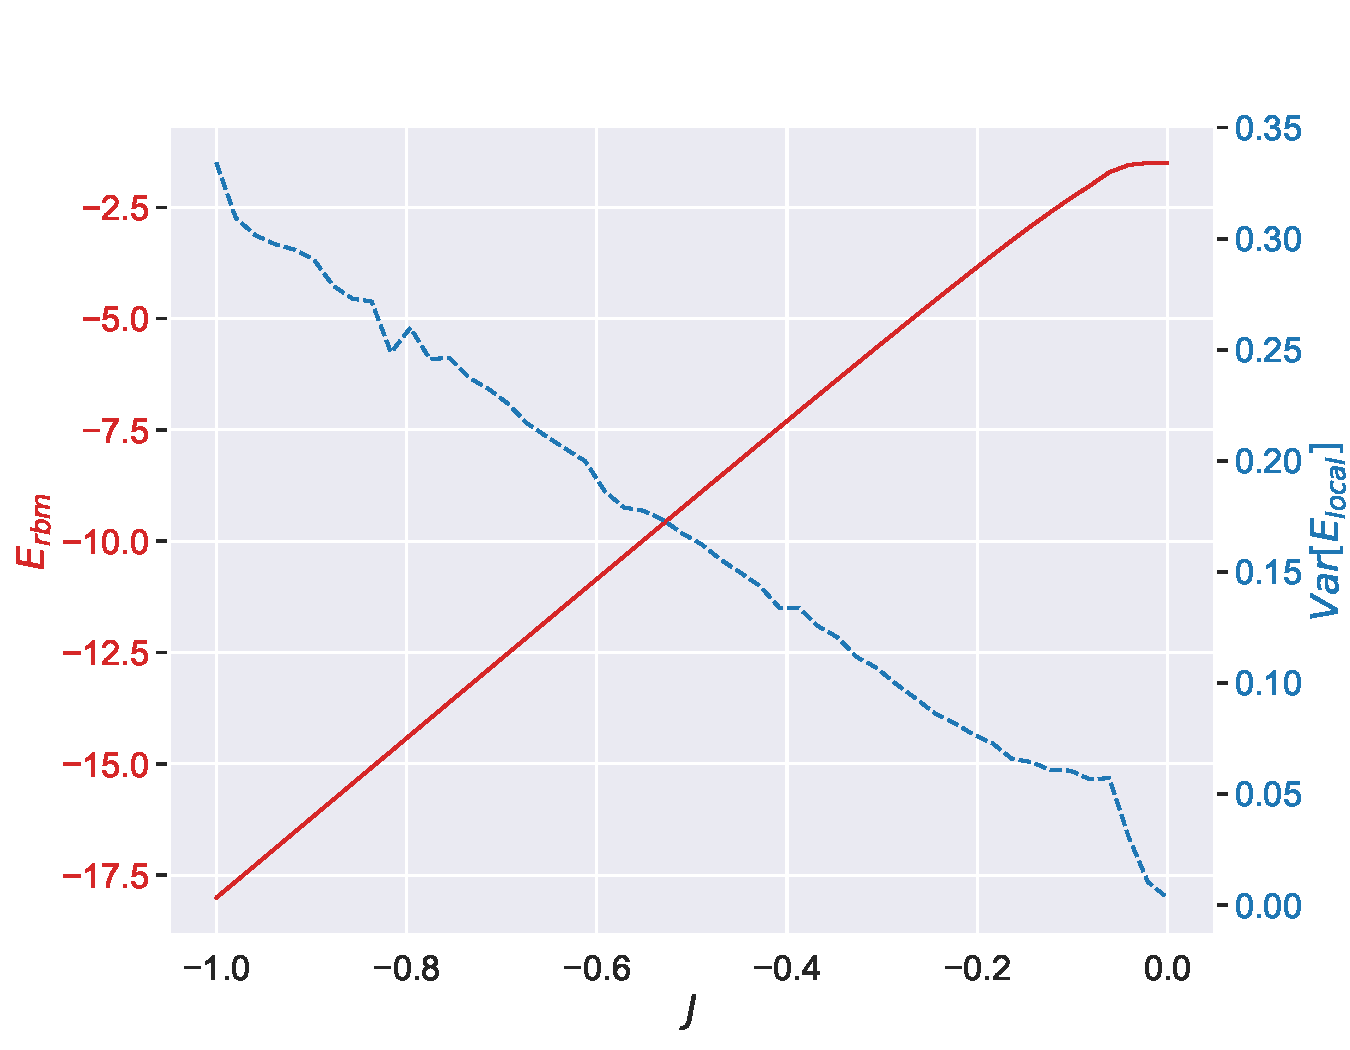
\includegraphics[width=0.95\textwidth]{Figures/Plots/Ising/[J][-1.0-0.0][e=500][n=9][L=-0.5]}
  \end{center}
  \caption{The variance of the restricted Boltzmann machine local energy output for the two-dimensional Ising model with $9$ lattice points, $N=3$ and $M=3$, and $L=-0.5$.}
\end{figure}
\subsection{The effect of \texorpdfstring{$L$}{L} on RBM prediction accuracy}

\begin{figure}[H]
  \begin{center}
    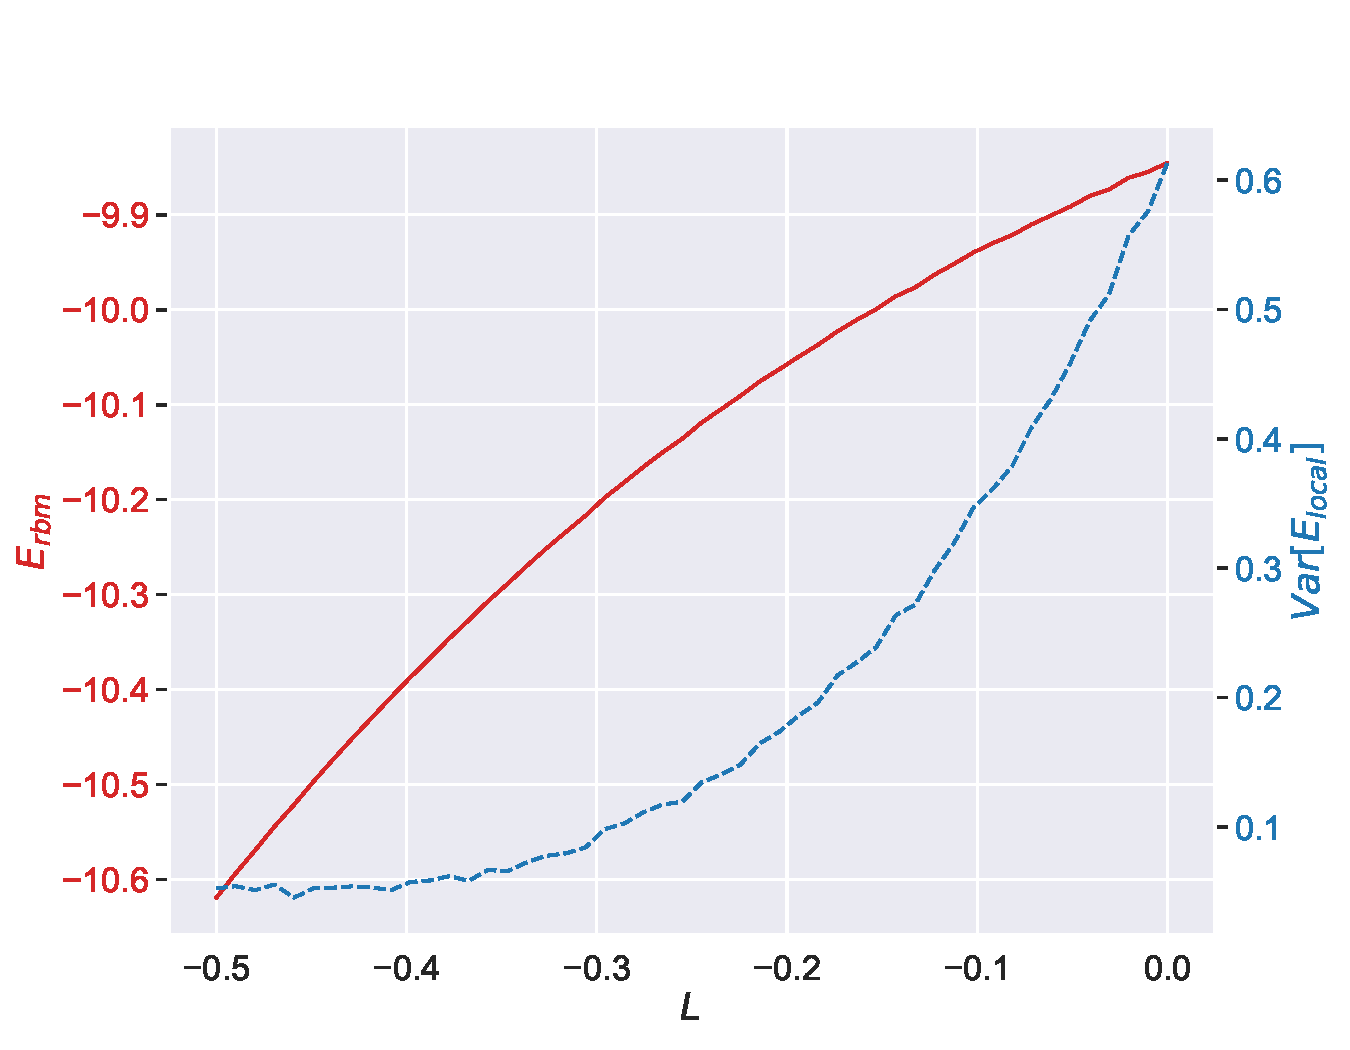
\includegraphics[width=0.95\textwidth]{Figures/Plots/Ising/[L][-0.5-0.0][e=500][n=10][J=-1]}
  \end{center}
  \caption{The variance of the restricted Boltzmann machine local energy output for the Ising model with $10$ lattice points and $J=-1$.}
\end{figure}

And with two dimensions

\begin{figure}[H]
  \begin{center}
    \includegraphics[width=0.95\textwidth]{Figures/Plots/Ising/[L][-0.5-0.0][e=500][n=9][J=-1]}
  \end{center}
  \caption{The variance of the restricted Boltzmann machine local energy output for the Ising model with $9$ lattice points, $N=3$ and $M=3$, and $J=-1$.}
\end{figure}

\subsection{Comparing computation time with diagonalization}

\chapter{The Heisenberg model}
\section{The Heisenberg model}
\subsection{The effect of \texorpdfstring{$J$}{J} on RBM prediction accuracy}
\subsection{The effect of \texorpdfstring{$L$}{L} on RBM prediction accuracy}
\subsection{Comparing computation time with diagonalization}

\chapter{The Pairing model}
\section{Convergence graph}

We first take a look at the converging predicted energy for the Pairing model with $P = 12$ energy levels included, $n = 6$ particle pairs, $\varepsilon = -0.3$ and $g = -1$.

\begin{figure}[H]
  \begin{center}
    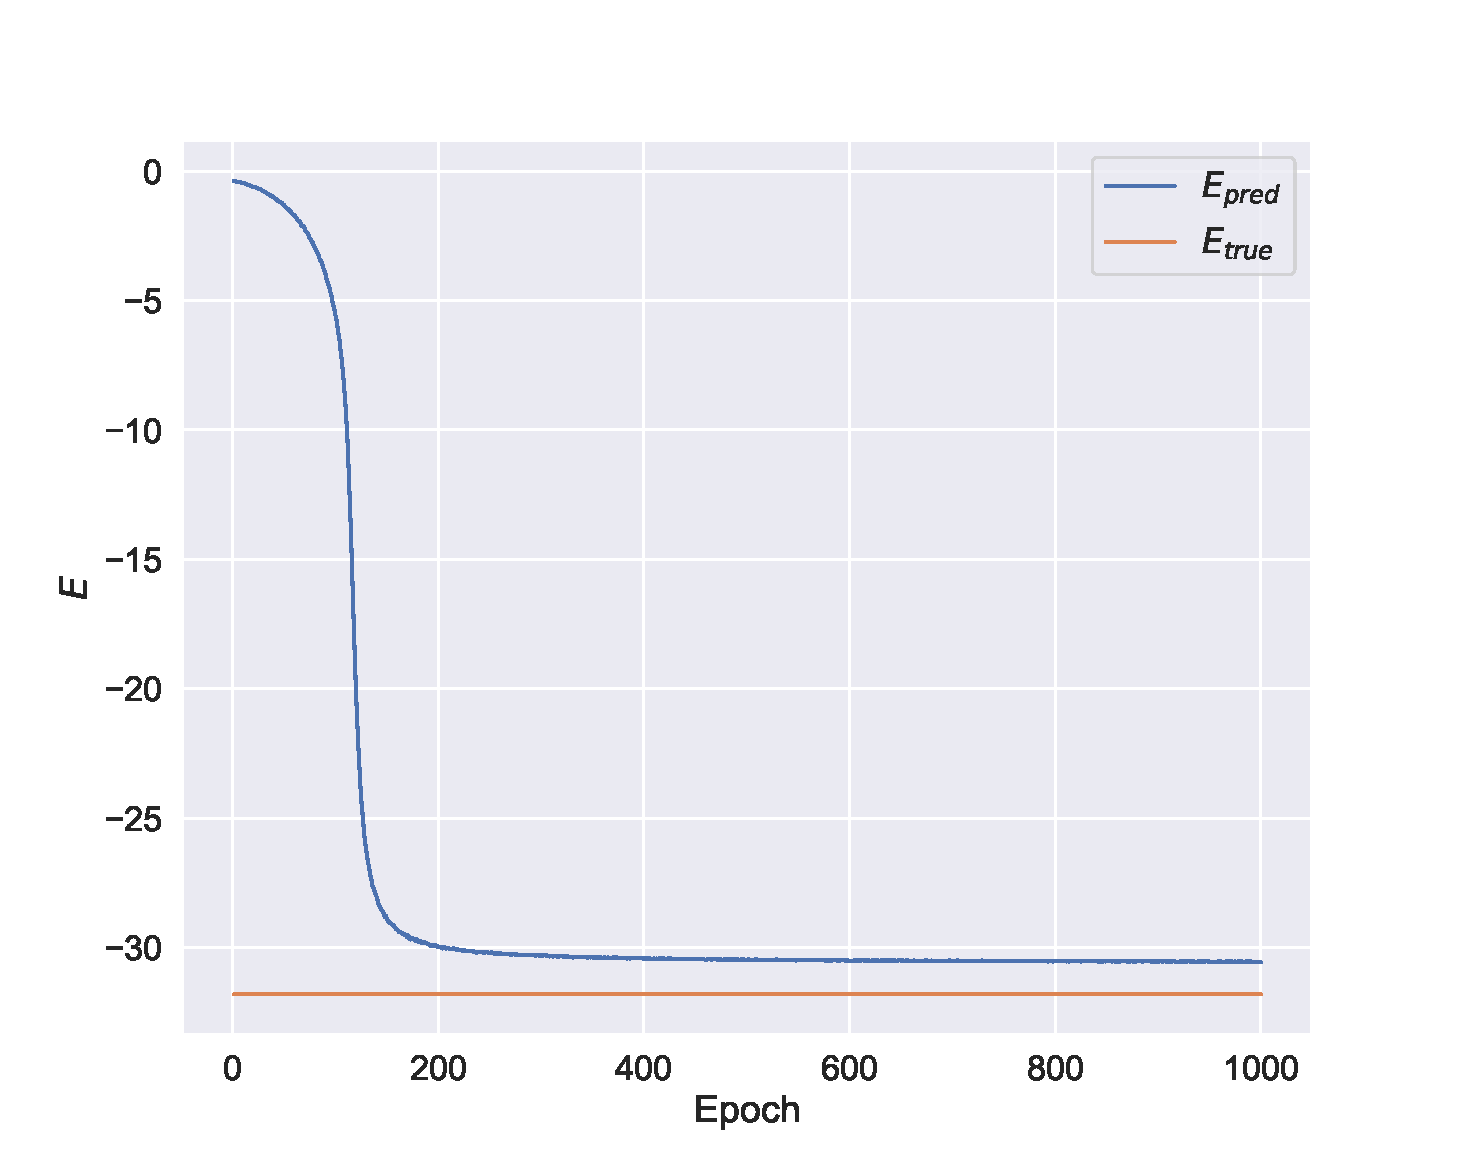
\includegraphics[width=0.95\textwidth]{Figures/Plots/Pairing/pairing_conv12}
  \end{center}
  \caption{The convergence graph of the RBM mean energy output for the Pairing model with particle pairs $n = 6$, levels $P=12$, and $\varepsilon=-0.3$ and $g=-1$.}
\end{figure}

Here we too have a small gap between the true ground state energy and the energy the RBM converge towards. This does as said earlier suggest that the RBM doesn't find the true wavefunction. 

\subsection{The effect of \texorpdfstring{$\varepsilon$}{epsilon} on RBM prediction accuracy}

Taking a look at the single particle energy variable $\varepsilon$ with a system of included energy levels $P = 10$, particles $n = 5$ and $g = 0$, we get:

\begin{figure}[H]
  \begin{center}
    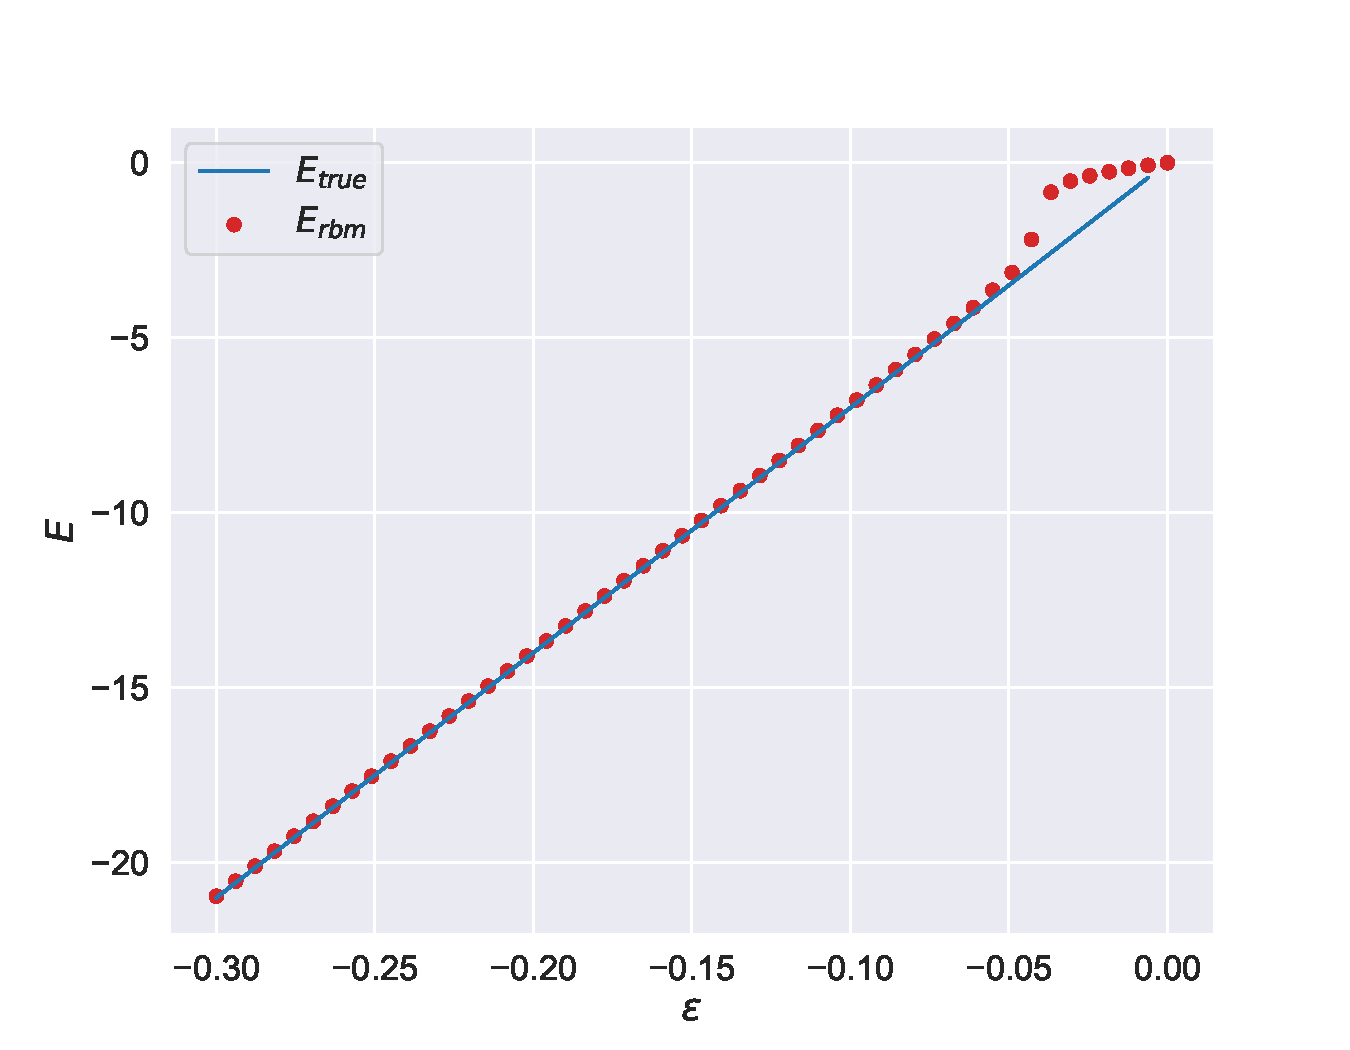
\includegraphics[width=0.95\textwidth]{Figures/Plots/Pairing/val-true[eps][-0.3-0.0][e=1000][n=10][n=5][g=0]}
  \end{center}
  \caption{The accuracy of the RBM for different values of $\varepsilon$ with number of particles as $n = 5$, levels $P=10$, and $g=0$.}
\end{figure}

The RBM seem to match the true ground state well for values up to $\varepsilon = -0.05$. At this point the RBM's predicted energy jumps closer to zero. For the Pairing model the Hamiltonian matrix does have large parts zeroed out, as many of the basis state are not accessible, and the RBM has to manage to find the accessible states by the lower local energy. Past a threshold a too small $\varepsilon$ may make these too difficult to distinguish.

\subsection{The effect of particle pairs on RBM accuracy}

We can then change the number of particle pairs instead, fixing $\varepsilon = -0.3$.

\begin{figure}[H]
  \begin{center}
    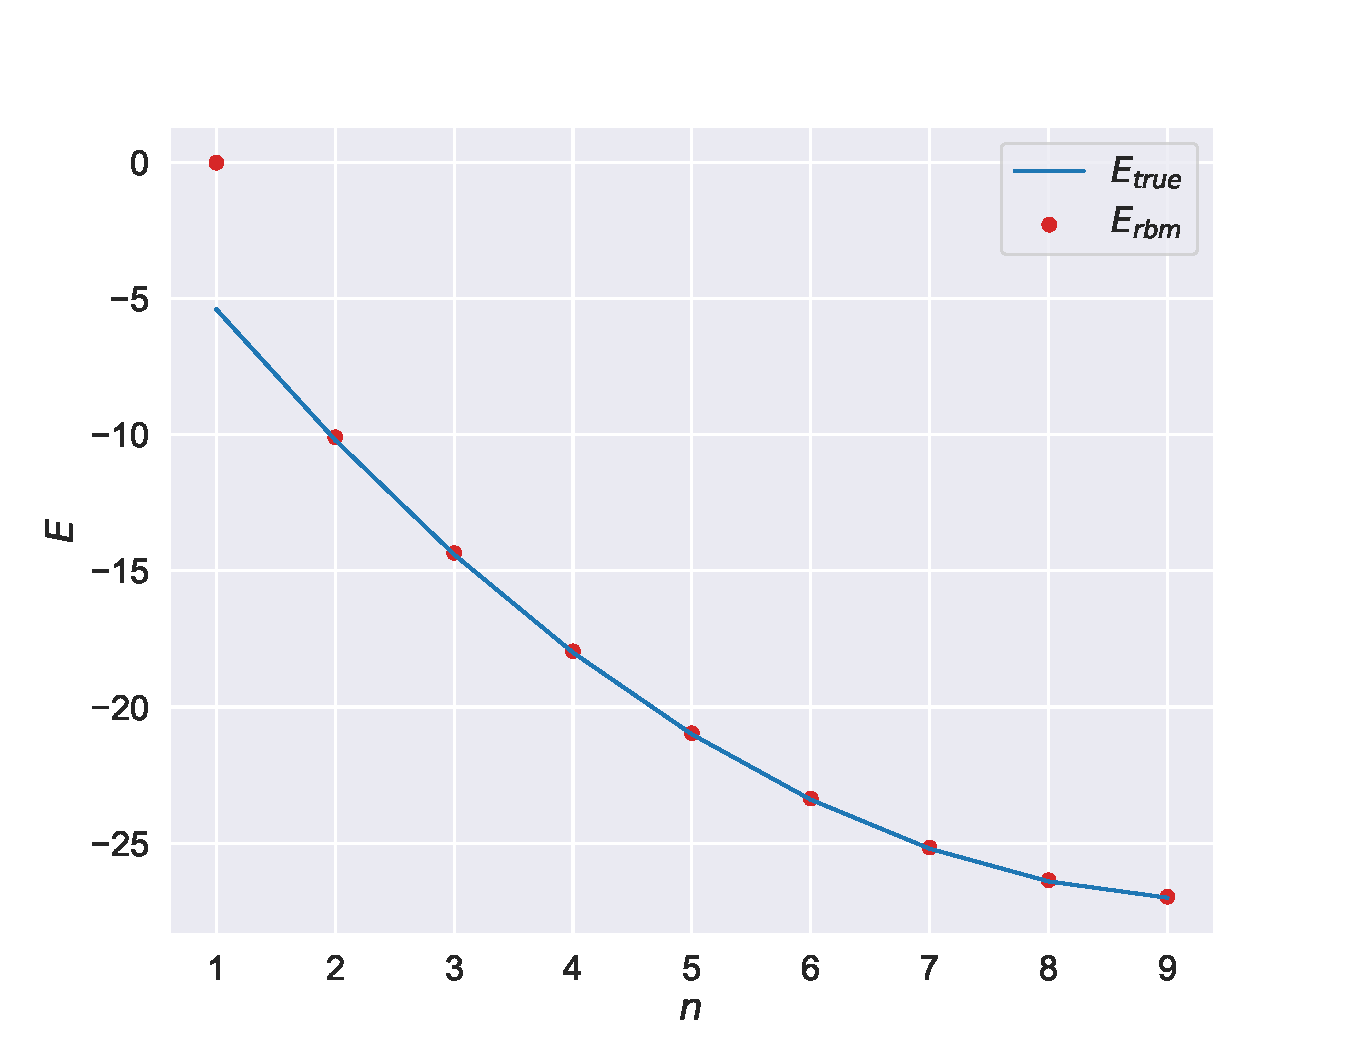
\includegraphics[width=0.95\textwidth]{Figures/Plots/Pairing/val-true[particles][1-9][e=1000][n=9][eps=-0.3][g=0]}
  \end{center}
  \caption{The accuracy of the RBM for different values of $\varepsilon$ with number of particles as $\eps = -0.3$, levels $P=10$, and $g = 0$.}
\end{figure}

The RBM predictors the ground state accurately for the different numbers of particle pairs except for $n=1$ where it defaults back to $E_{rbm} = 0$. A cause may be that for the case of only one particle pair the Hamiltonian matrix contains almost only zeros, so the RBM struggles to find the accessible states. This begs the question why the RBM manages to predict the ground state energy accurately for the $n=9$ case, where the number of non-accessible basis states are the same as for $n=1$. As suggested previously this may come from that the energy for $n=9$ case is of higher absolute value, such that additions of the accessible basis states in the machine state has a larger effect on the machine state energy during the learning process.

\subsection{The effect of \texorpdfstring{$g$}{g} on RBM prediction accuracy}

\begin{figure}[H]
  \begin{center}
    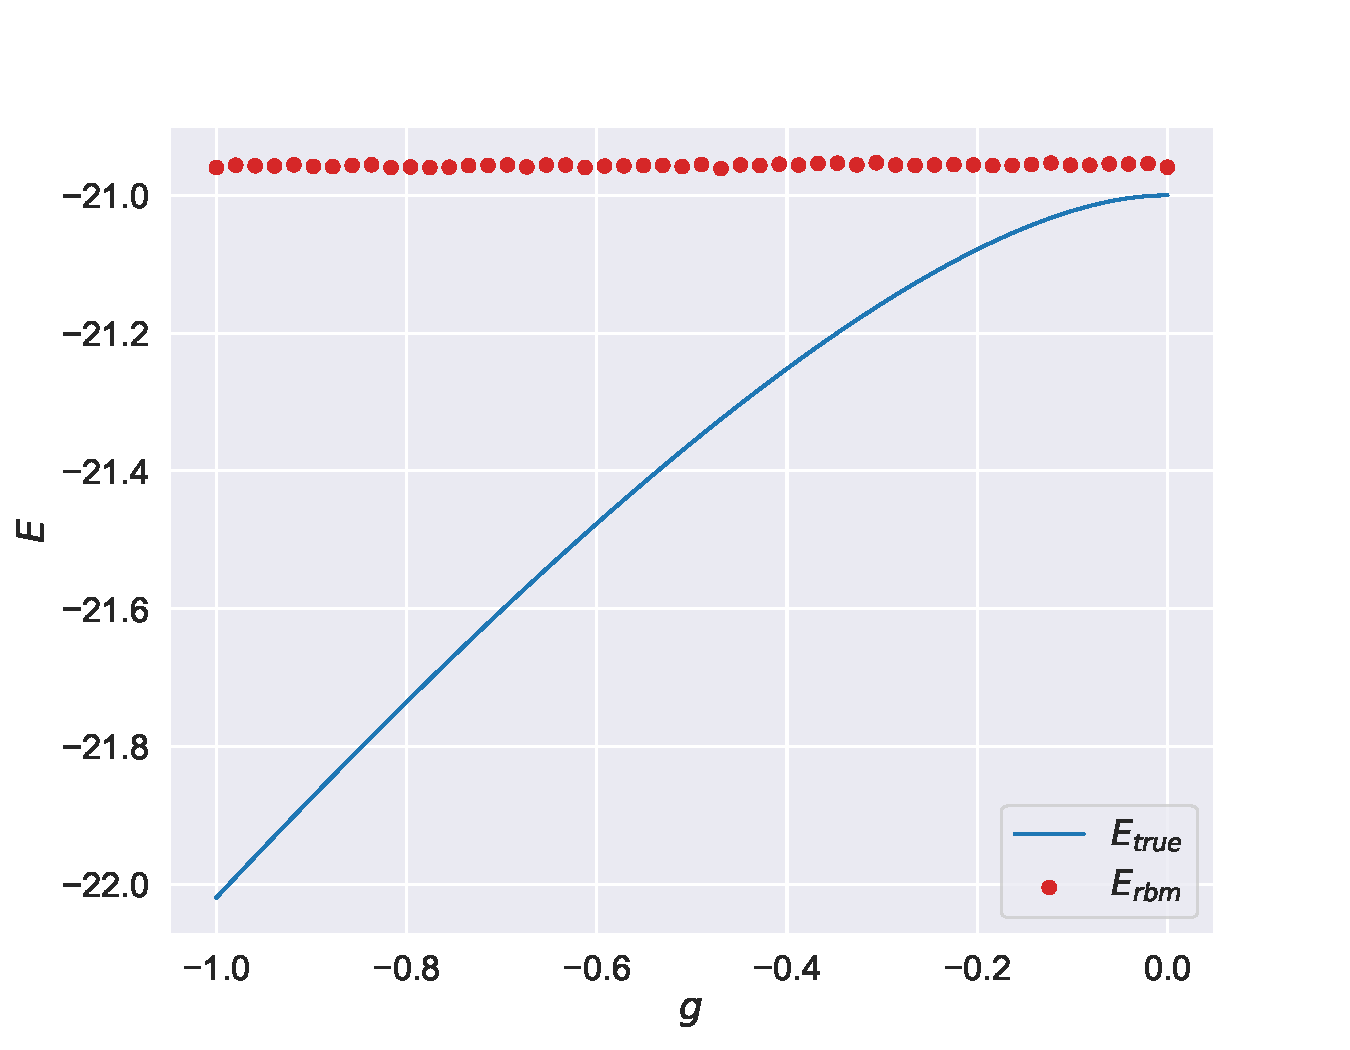
\includegraphics[width=0.95\textwidth]{Figures/Plots/Pairing/val-true[g][-1.0-0.0][e=1000][n=10][n=5][eps=-0.3]}
  \end{center}
  \caption{The accuracy of the RBM for different values of $\varepsilon$ with number of particles as $\eps = -0.3$, $n=5$ and levels $P=10$.}
\end{figure}

It is clear that the restricted Boltzmann machine completely ignores the $g$ interaction strength of the Pairing model. A reason for this may be that it finds the non-interactive ground state energy, but then struggles to escape the local minima or that the local energy average becomes too sensitive to small changes to the machine state.


\chapter{Computation time}
\section{Comparing implementation and diagonalization}

We also want to test our RBM implementation's computation time against the standard diagonalization algorithms. It is expected that the RBM only stands a chance to overtake these algorithms at large matrix sizes. For the Lipkin model we have used the symmetry of the total spin to to essentially reduce the size of the Hamiltonian. On the other hand the Pairing model Hamiltonian matrix could also be reduced by the fact that large parts of it is only zeros. Because of this we will look at the case of the Ising and Heisenberg models, but with the Ising model Hamiltonian only as the size evolves by $2^N\times 2^N$ for both cases. With the Ising model using $100 000$ Monte Carlo cycles each epoch of the learning process, with $500$ epochs in total, we get the following:

\begin{figure}[H]
  \begin{center}
    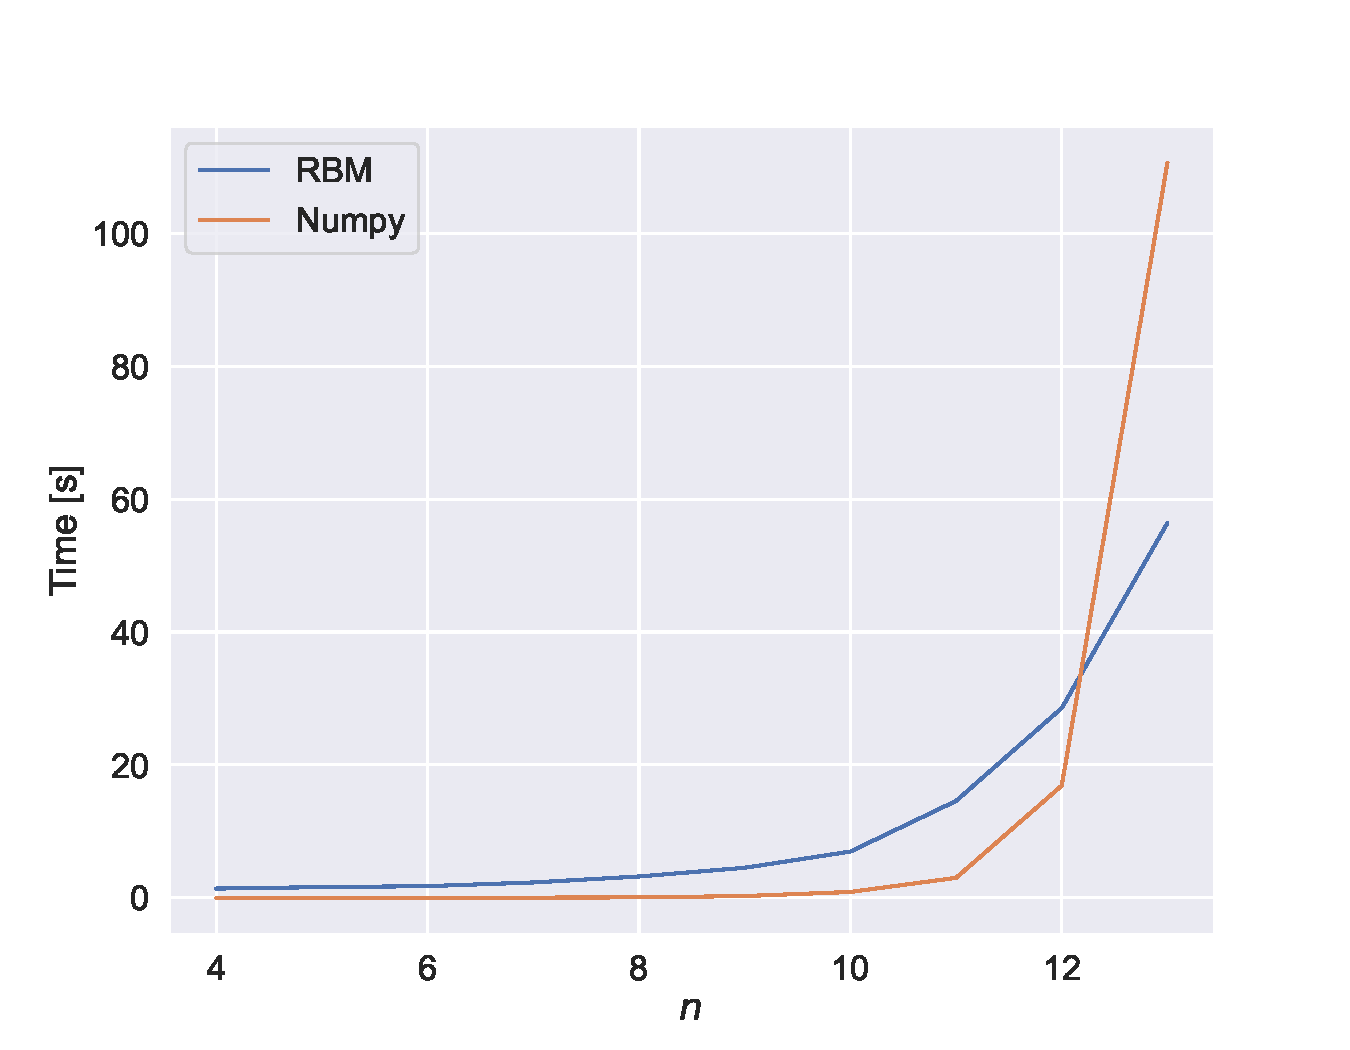
\includegraphics[width=0.95\textwidth]{Figures/Plots/Ising/[particles][4-13][e=500][J=0.3][L=-0.4]}
  \end{center}
  \caption{The computation time for finding the ground state energy for the Ising model with our implemented RBM compared with the time used by traditional diagonalization algorithms. Each data point is averaged over twenty runs. The diagonalization method used is \mintinline{python}{numpy.linalg.eigvals}.}
\end{figure}

We see that for the lower particle counts the standard diagonalization technique is superior, but as the Hamiltonian matrix size increases the RBM overtakes it at our last data point $n=13$. Here we use a algorithm that is for diagonalizing a general square matrix, but a more efficient version could be used, \mintinline{python}{numpy.linalg.eigvalsh}, as we are really dealing with sparse matrices. Comparing the RBM with the more efficient diagonalization algorithm we get:

\begin{figure}[H]
  \begin{center}
    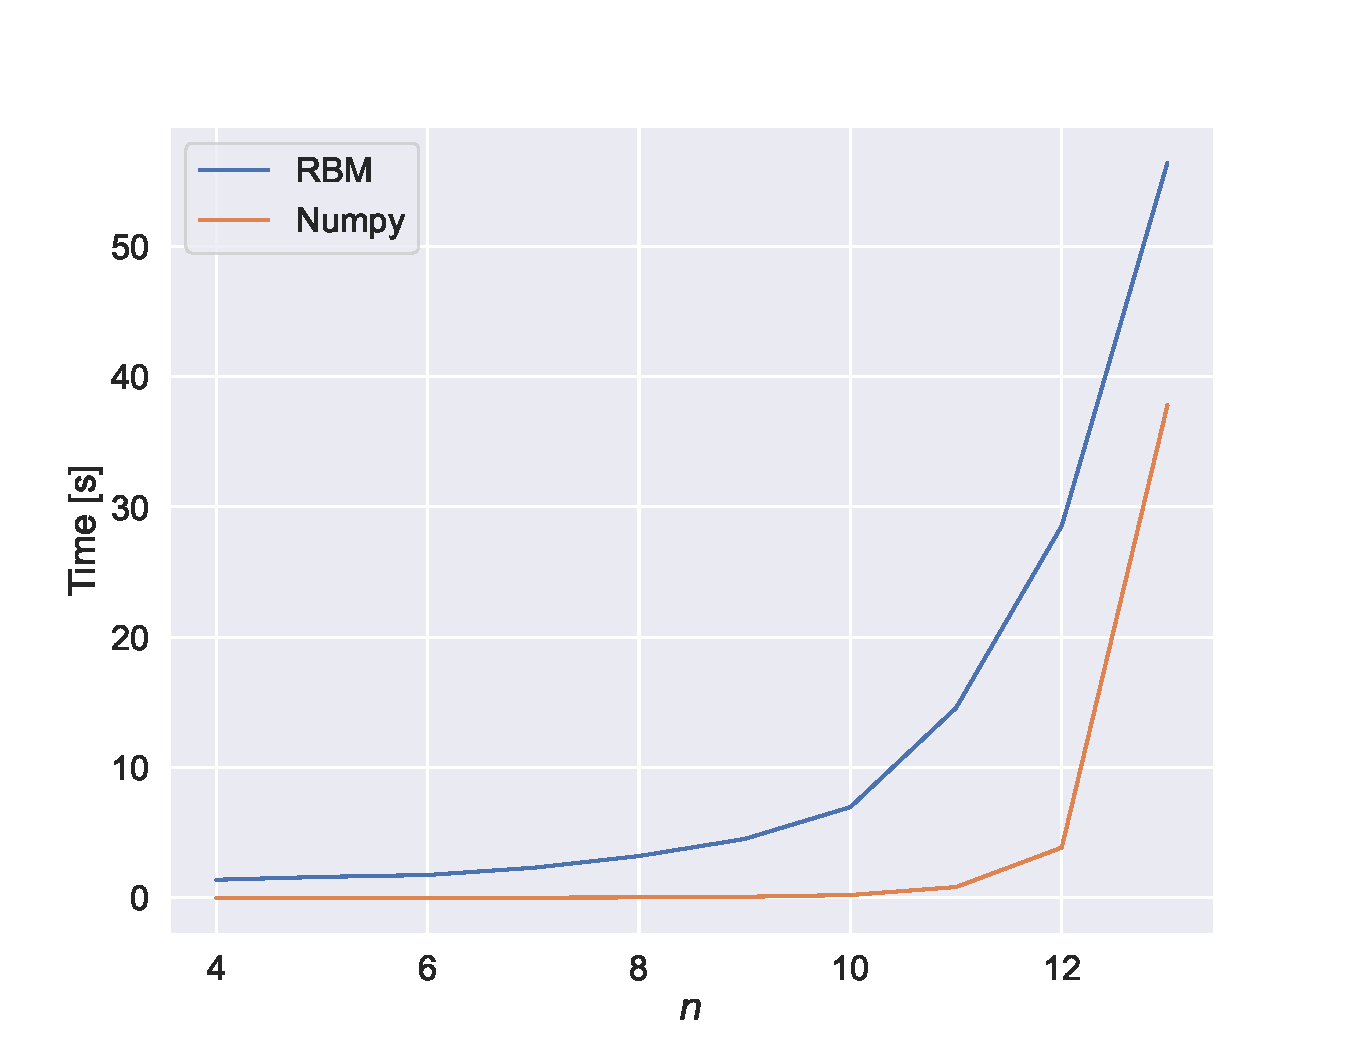
\includegraphics[width=0.95\textwidth]{Figures/Plots/Ising/[particles][4-13][e=500][J=0.3][L=-0.4][eigvalsh]}
  \end{center}
  \caption{The computation time for finding the ground state energy for the Ising model with our implemented RBM compared with the time used by traditional diagonalization algorithms. Each data point is averaged over twenty runs. The diagonalization method used is \mintinline{python}{numpy.linalg.eigvalsh}.}
\end{figure}

And we see that the RBM has once again fallen behind. It does seem like the \mintinline{python}{eigvalsh} algorithm still has a steeper incline at the $n=13$ mark, so one can assume here the RBM implementation would overtake it at even greater system sizes.




\chapter{Comparing Metropolis-Hasting algorithm and the Gibbs sampling method}
\section{Comparing conditional acceptance and the Gibbs sampling method.}

The Metropolis-Hastings sampling algorithm uses a conditional acceptance ratio. The Gibbs sampling method, which is what we have mostly used throughout this thesis, removes this condition and accepts every proposed sample state. With Gibbs sampling we can vectorize the process, resulting in a substantial decrease in computation time. Here we would like to see if the acceptance criteria, based on the RBM's internal energy, can improve prediction accuracy by giving a better approximation of the machine state. 

\vspace{\baselineskip}

\def \mgJ {4}
\def \mgeps {1.5 - \frac{\sqrt{3}}{2}}
\def \mgV {-1}
\def \mgW {0}
\def \mgk {1}
\def \mgC {5*10^5}

For comparison we will use the Lipkin model with $J= \mgJ$ and $\varepsilon = \mgeps$, $V= \mgV$, and $W = \mgW$. We first compare the evolution of the methods accuracy as the number of samples, or the number of Monte Carlo cycles, increases. The number of Gibbs cycles are here set to $k = \mgk$.

\begin{figure}[H]
  \begin{center}
    \includegraphics[width=0.95\textwidth]{}
  \end{center}
  \caption{The error of two RBMs where one uses the Gibbs sampling method, and the other uses a conditional acceptance criteria of the RBM's internal energy. The number of Gibbs sampling cycles is $k = \mgk$. The quantum system is the Lipkin model with $J= \mgJ$ and $\varepsilon = \mgeps$, $V= \mgV$, and $W = \mgW$.}\label{fig:met_hast_1}
\end{figure}

We then see if the number of Gibbs sampling cycles makes a difference:

\begin{figure}[H]
  \begin{center}
    \includegraphics[width=0.95\textwidth]{}
  \end{center}
  \caption{The error of two RBMs where one uses the Gibbs sampling method, and the other uses a conditional acceptance criteria of the RBM's internal energy. The number samples is set to $\mgC$. The quantum system is the Lipkin model with $J= \mgJ$ and $\varepsilon = \mgeps$, $V= \mgV$, and $W = \mgW$.}\label{fig:met_hast_2}
\end{figure}







